% LaTeX file for Chapter 03


\chapter{Results}

\section{Exploratory Data Analysis}

\subsection{Mouse kidney cells}
The first data set stems from a paper that investigates potential cellular targets of kidney disease in mice \citep{mouse_cells}. The authors isolated and sequenced a total of 57'979 cells from whole kidney cell suspensions (one kidney per mouse) derived from seven healthy male mice using droplet-based single-cell RNA sequencing. The samples were labeled as: normal1, normal2, normal3, normal4, Ksp-cre-GFP, Scl-cre-GFP and Pod-cre-GFP. After quality controls the authors used clustering analysis on 43'745 cells to classify 16 major cell clusters. Further, cell-type specific marker genes were used to identify the cell clusters. In the end, the authors identified 21 major cell types by quantitative gene expression. For our work, we decided to use the raw data from the four samples that were labeled as categorized as normal to ensure the biological replicability between the samples.

We used the \emph{alevin-fry} pipeline to quantify the raw single-cell RNA sequencing data for further use in the R programming environment. Quality control is a crucial stage in data pre-processing as low-quality libraries can contribute to misleading results in downstream analyses \citep{OSCA}. The main problems that arise from neglected quality control are the following: First, low-quality libraries can form their own distinct clusters which in the worst-case scenario are generated solely based on similarities in the damage-induced expression profiles. Second, principal component analysis will capture differences between mostly on quality rather than biology. Therefore, we filtered lowly abundant genes and low-quality cells to mitigate said problems to improve interpretability of the results. 

To identify low-quality cells, cell-specific QC metrics were calculated with the \emph{perCellQCMetrics} function from the \emph{scater} R package \citep{scater}. These metrics include the total number of expressed genes, the overall count across all genes, and the fraction of counts assigned to control genes such as mitochondrial genes. By setting a specific threshold on per-cell QC metrics, high-quality cells can be retained. In our setting, outliers are defined as cells with library sizes more than two median absolute deviations away from the median library size. Figure \ref{fig:QC} summarizes the process from unprocessed to processed single-cell experiment. After filtering, the data set consists of 23'543 cells and 18'537 genes. Next, we used the \emph{singleR} function from the \emph{singleR} R package \citep{singleR} for cell-type annotation. Cell-type annotation is important to determine what biological state is represented by cell clusters which helps the interpretability of the results and their implications \citep{OSCA}. \emph{singleR} is a method that assigns labels based on the reference samples with the highest Spearman rank correlation while only using marker genes between pairs of labels to focus on the relevant differences between cell types \citep{singleR}.

\begin{figure}[!htb]
\begin{center}
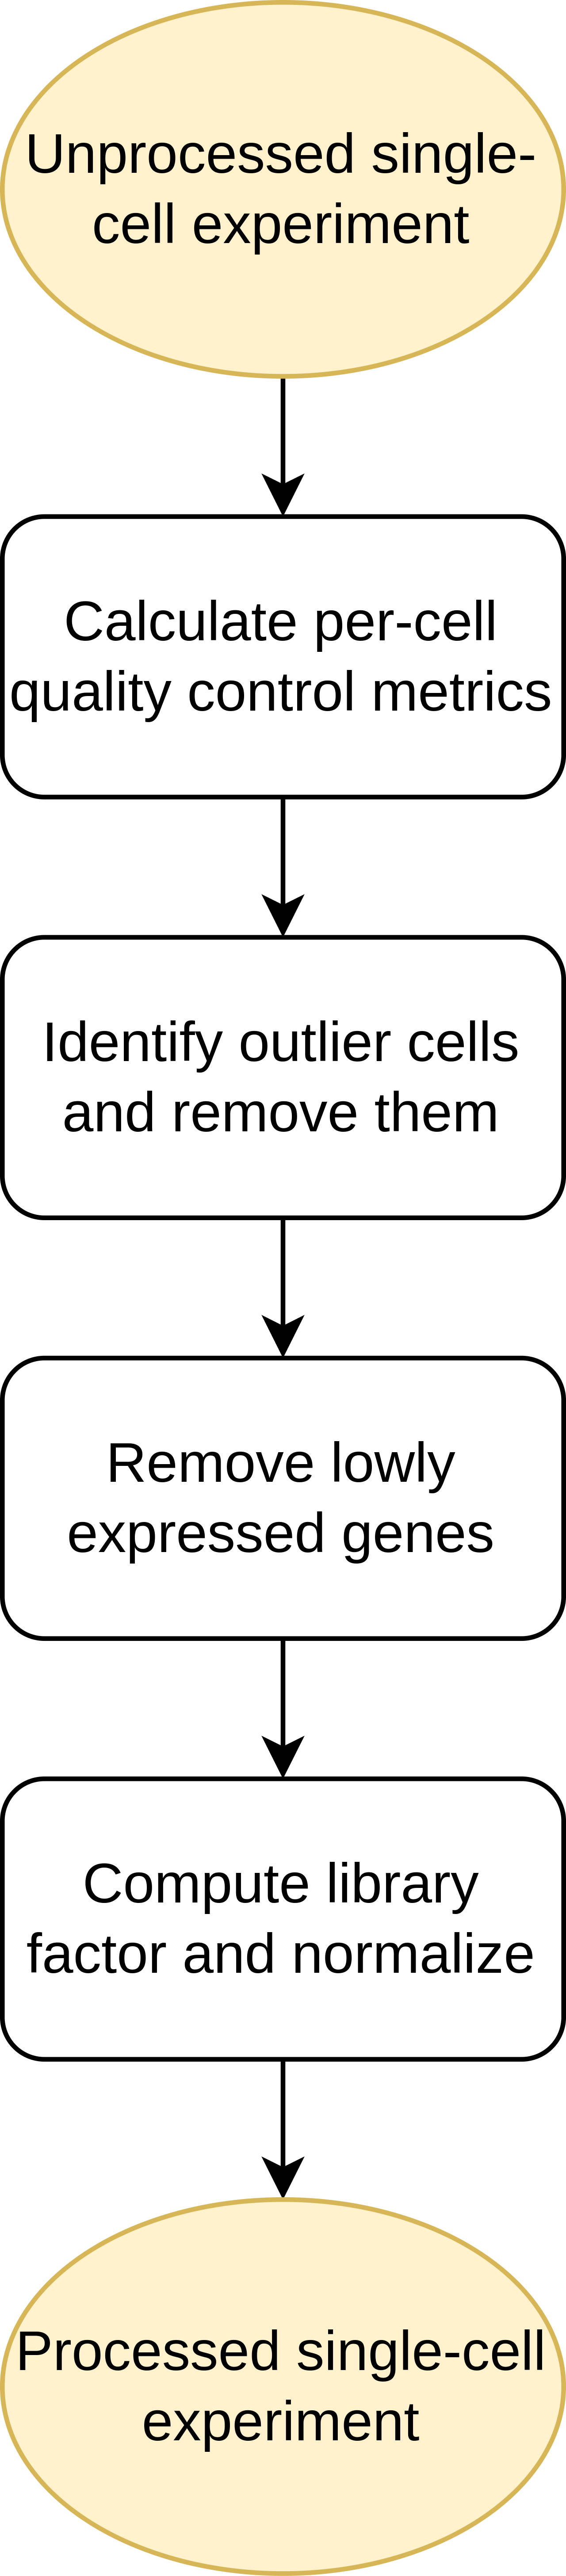
\includegraphics[width=1.5in,height=6in]{figure/qc.png}
\end{center}
\caption{Quality control process from unprocessed, raw to processed, filtered single-cell experiment}
\label{fig:QC}
\end{figure}
\FloatBarrier

\begin{figure}[!htb]
\begin{center}
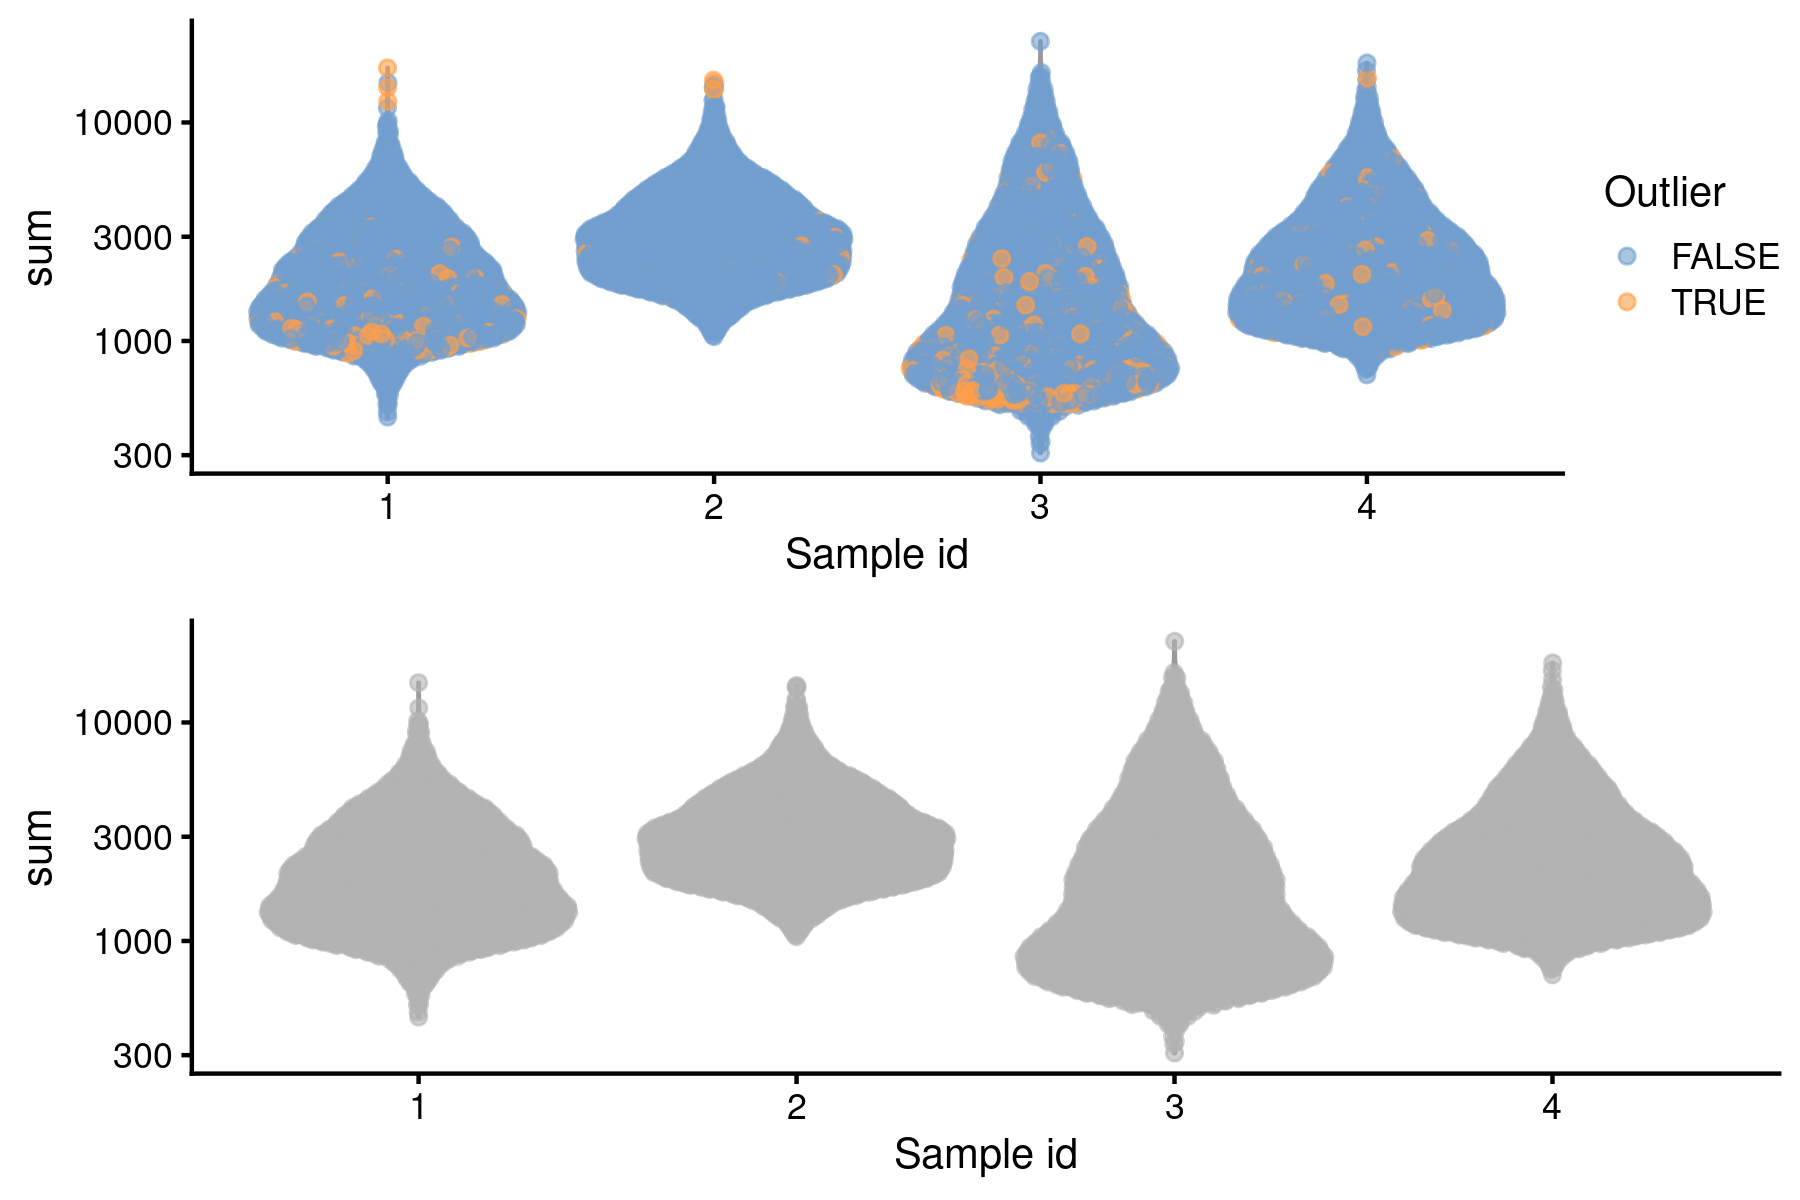
\includegraphics{figure/kidney_mouse/qc_mouse.png}
\end{center}
\caption{Violin plots reporting the number of UMI counts in the mouse kidney data. Top: before QC. Colours indicate whether a cell is identtifie as an outlier (orange) or not (blue). Bottom: after QC.}
\label{fig:QC_mouse}
\end{figure}
\FloatBarrier


Figure \ref{fig:UMAP_mouse_sample}  shows that the cells largely overlap based on the UMAP representation 

\begin{figure}[!htb]
\begin{center}
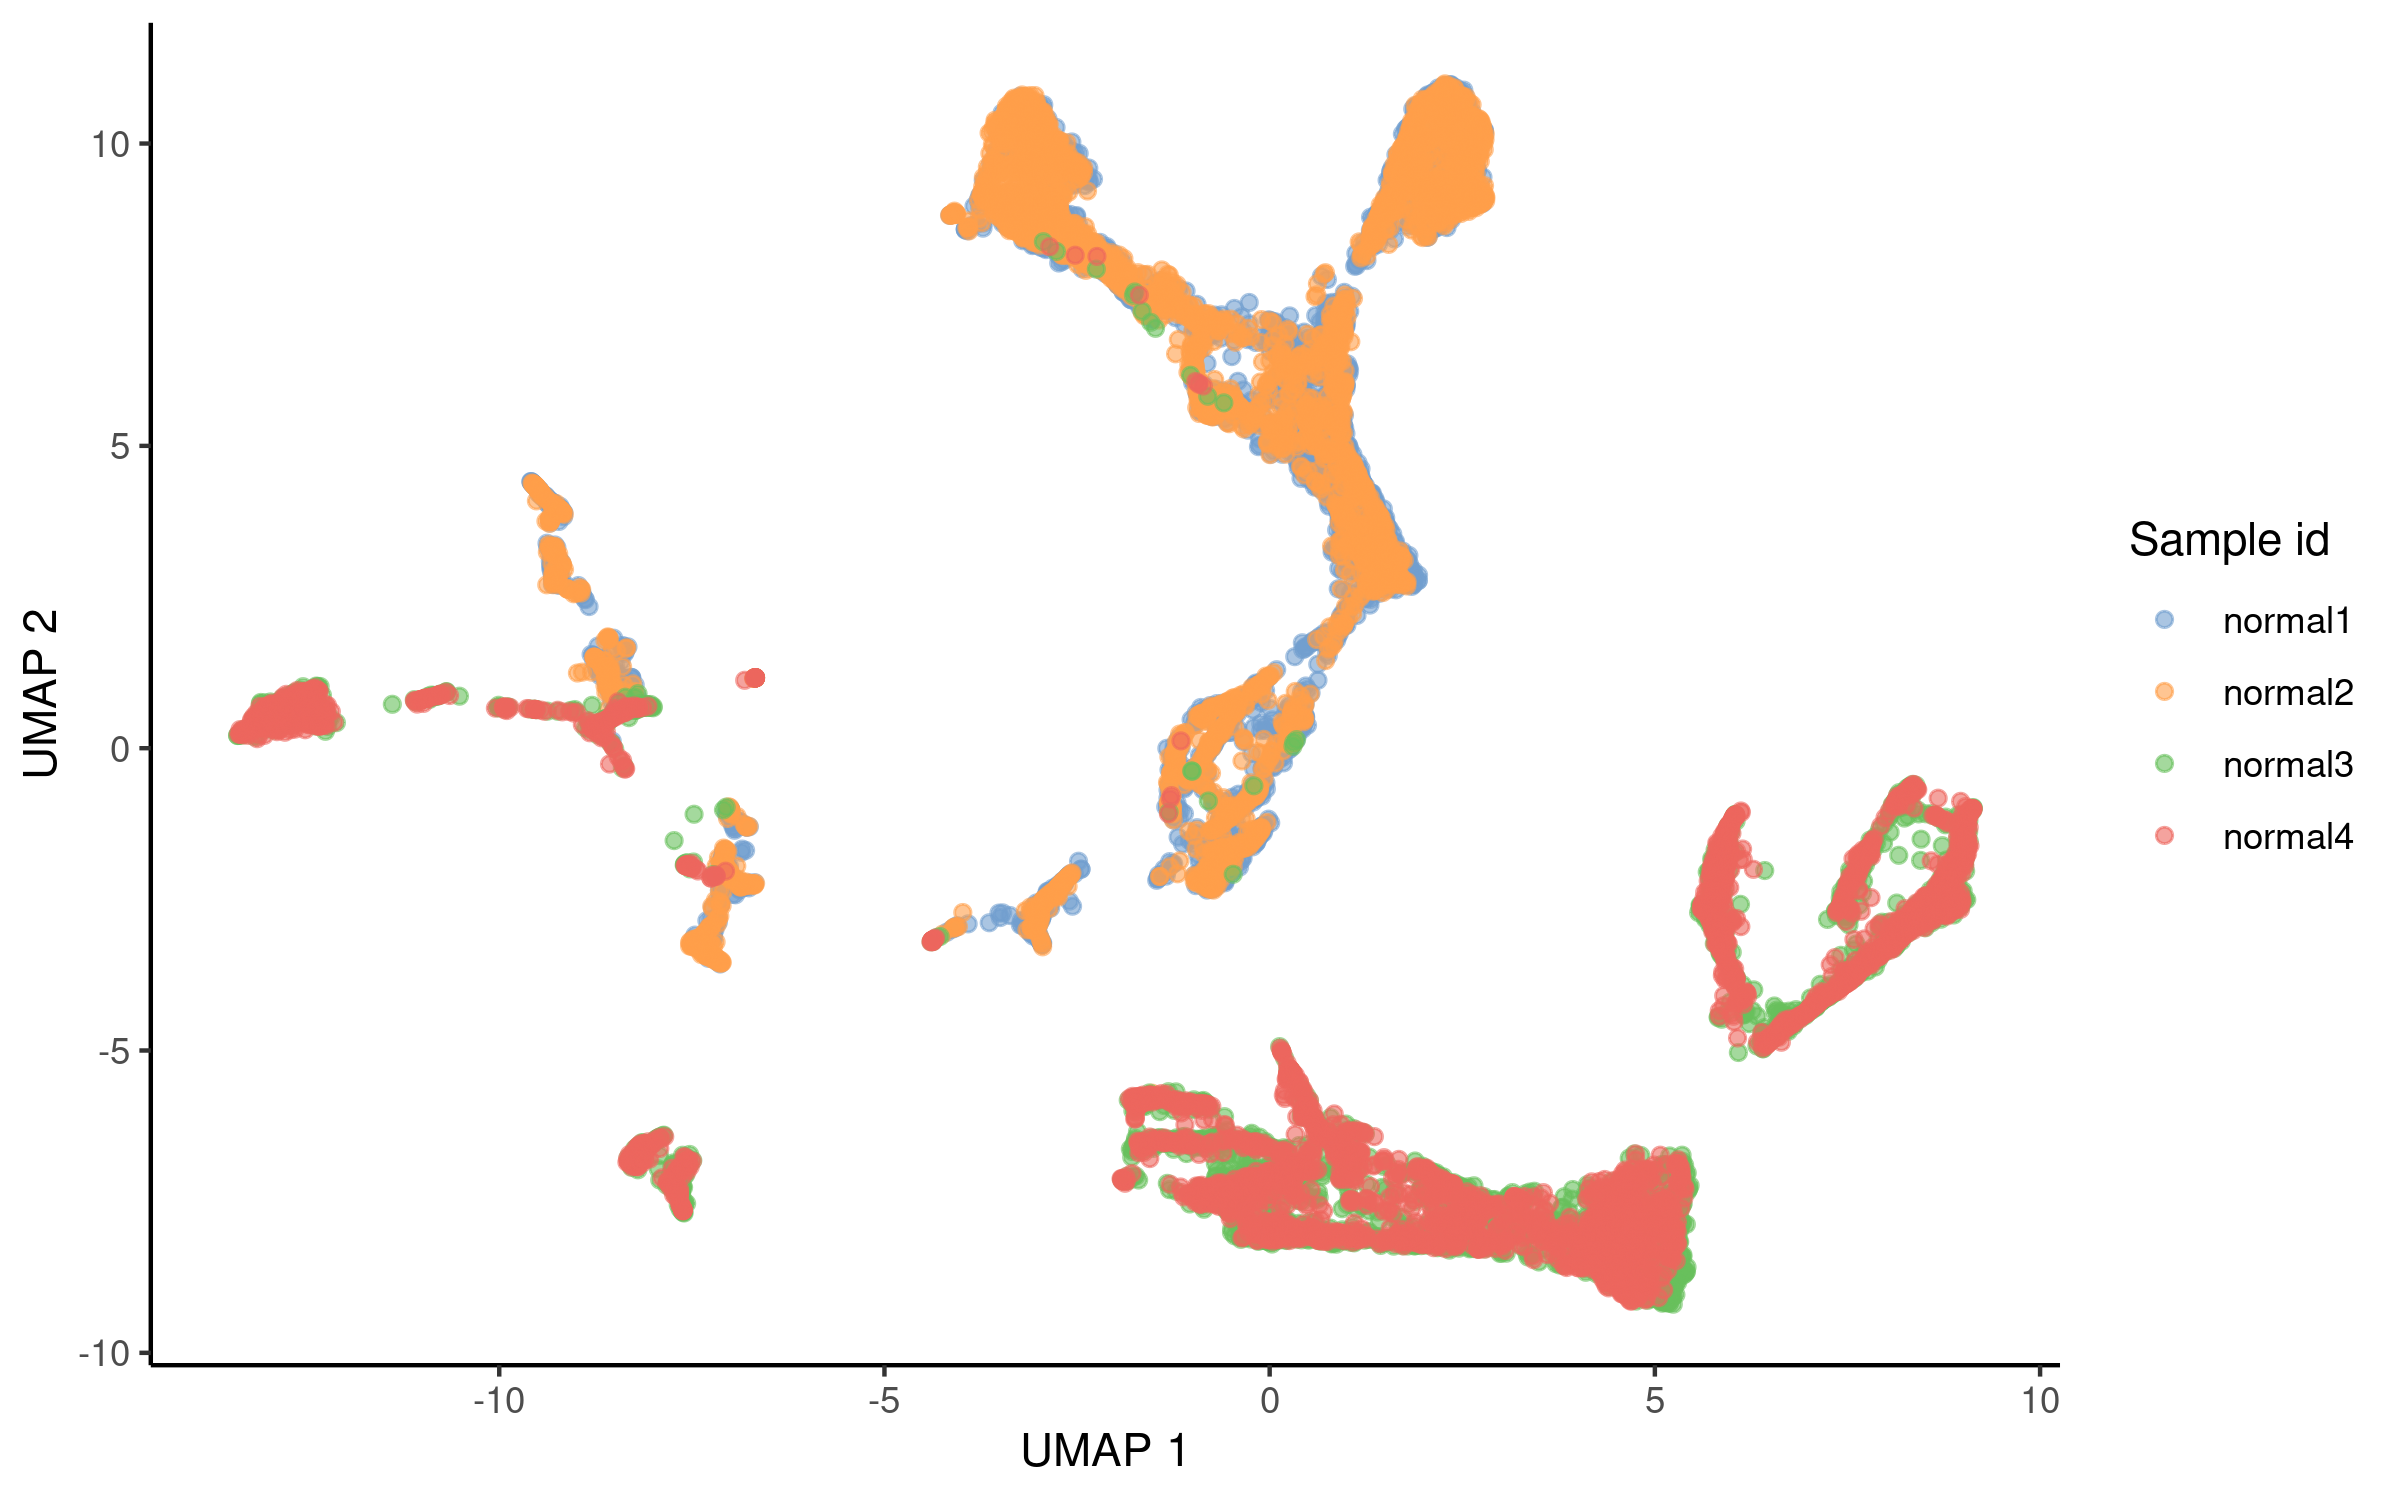
\includegraphics[width=6in,height=4in]{figure/kidney_mouse/UMAP_sample_id.png}
\end{center}
\caption{UMAP representation of the mouse kidney cells based on the sample coloured by sample id}
\label{fig:UMAP_mouse_sample}
\end{figure}
\FloatBarrier

Figure \ref{fig:UMAP_mouse_cell_type} shows 

\begin{figure}[!htb]
\begin{center}
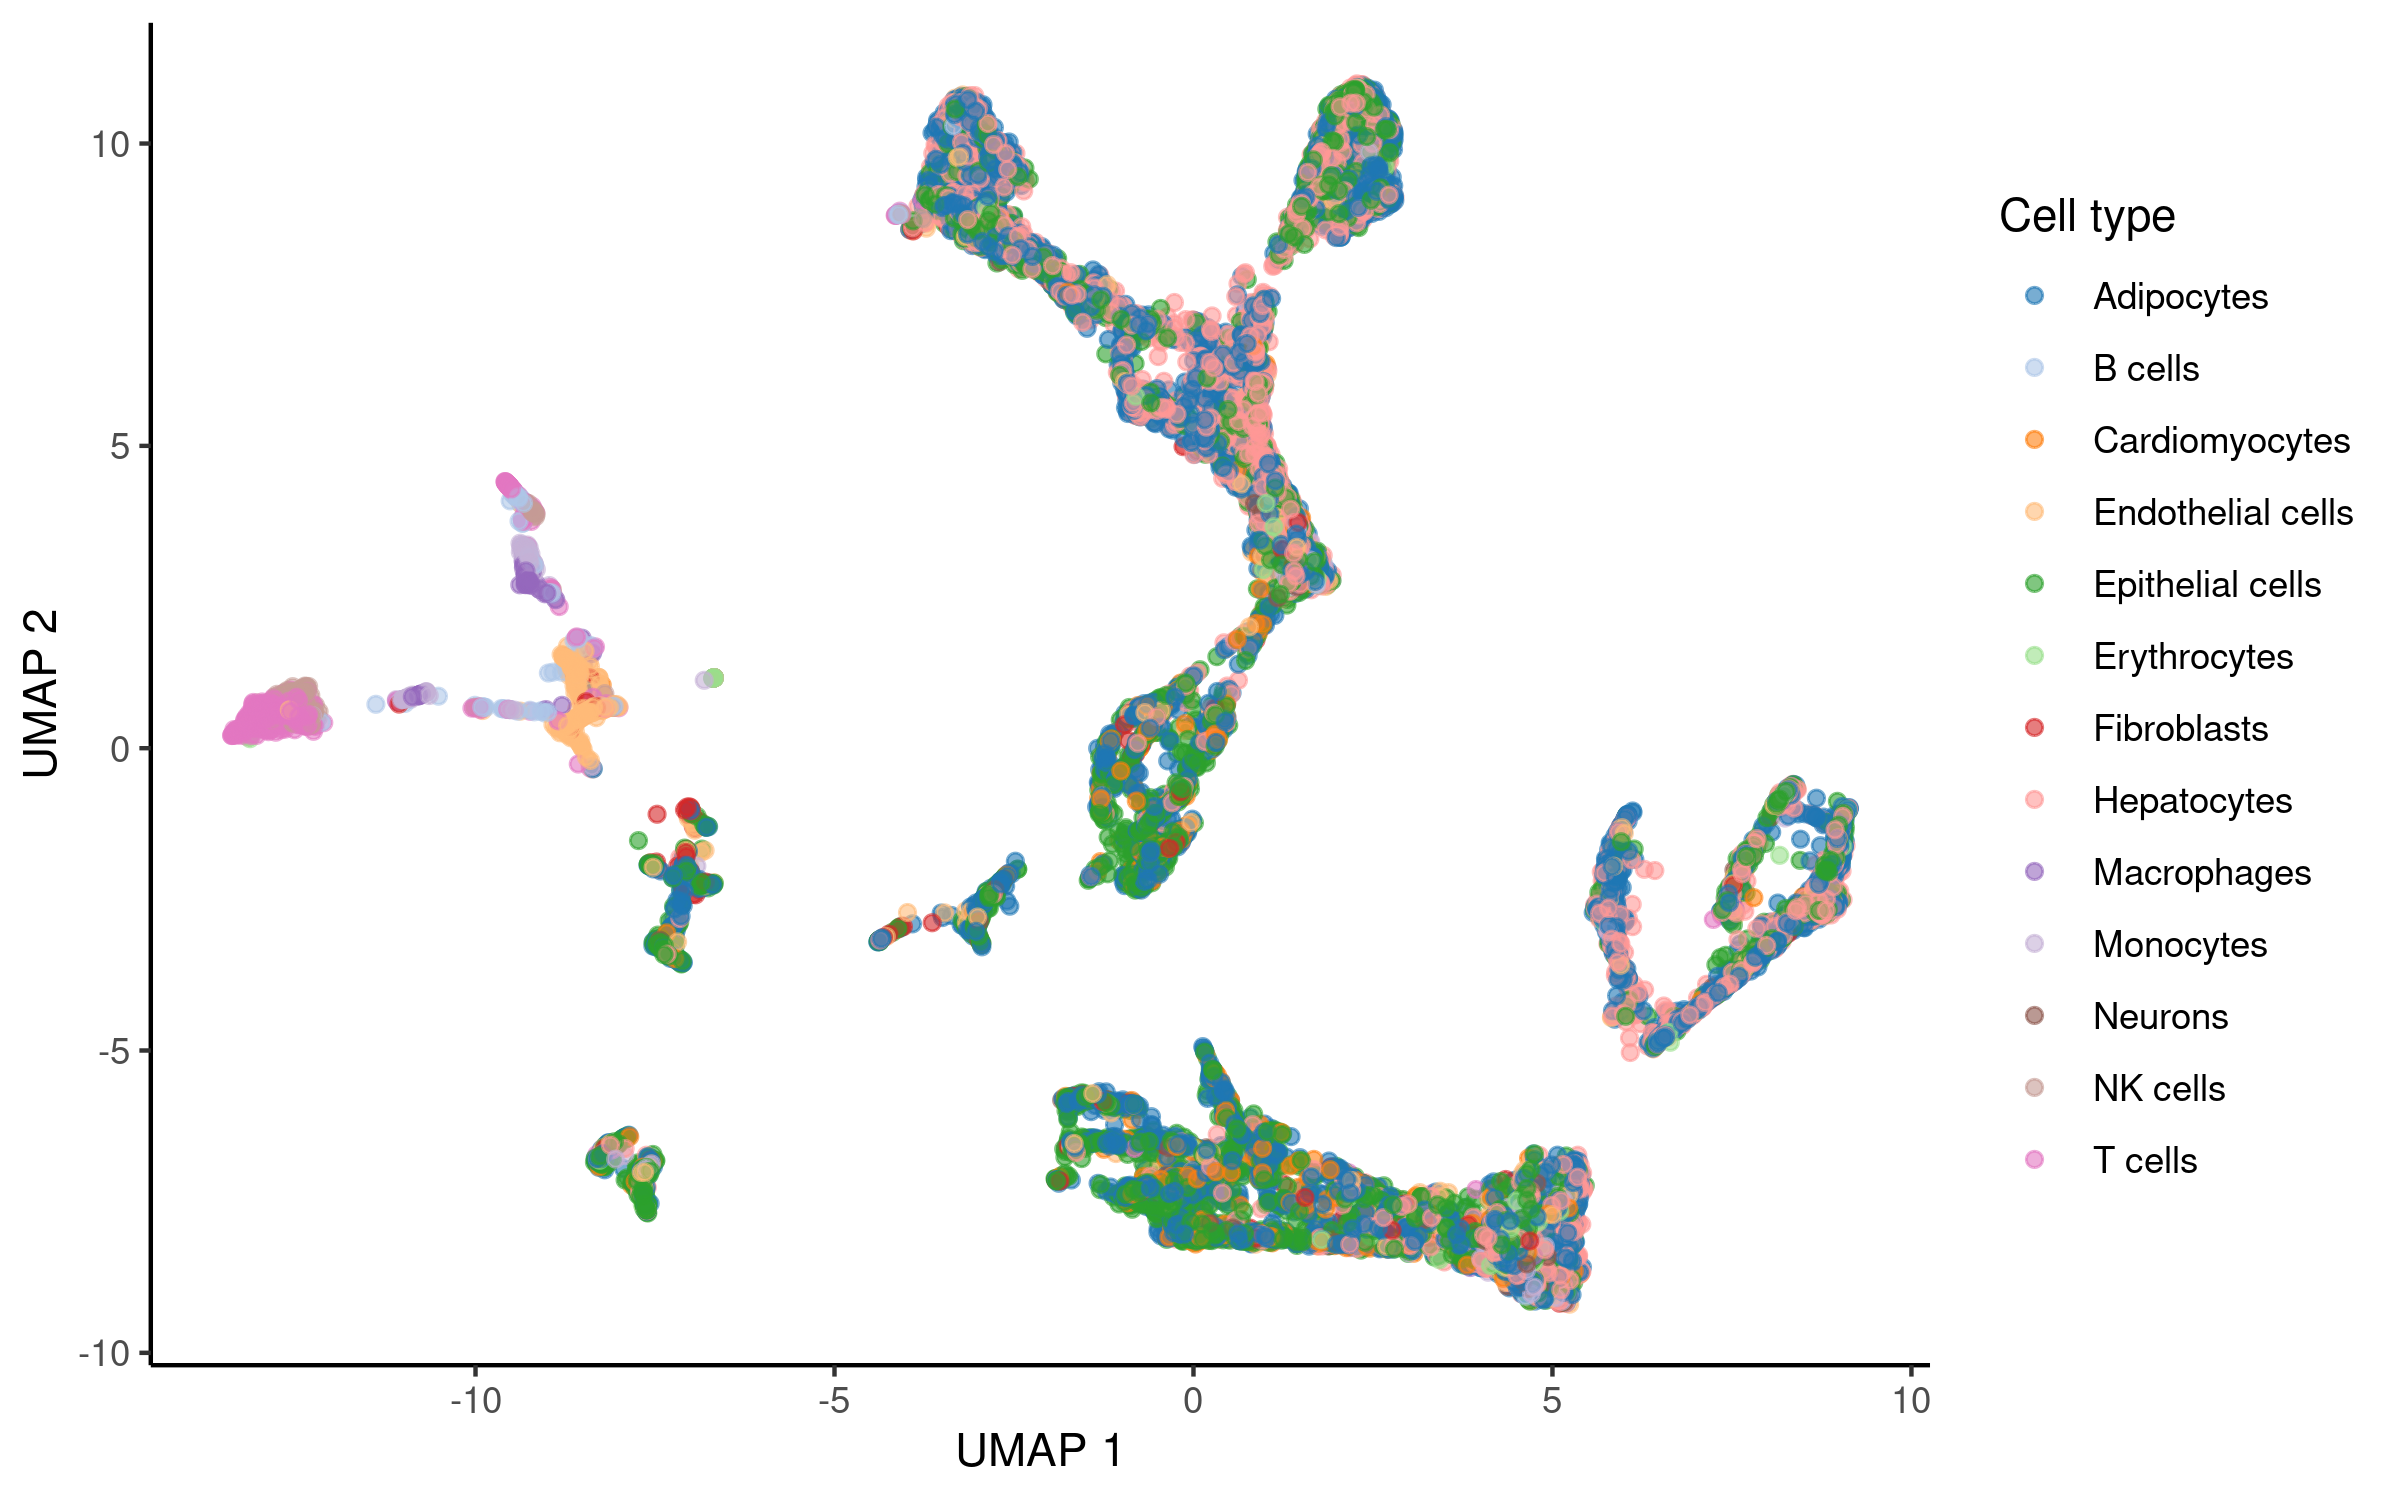
\includegraphics[width=6in,height=4in]{figure/kidney_mouse/UMAP_cell_type.png}
\end{center}
\caption{UMAP representation of the counts based on the cell type}
\label{fig:UMAP_mouse_cell_type}
\end{figure}
\FloatBarrier

\subsection{Human brain organoids}
The second data set we investigated


\citep{brain_organoids}

\section{Simulation study on the mouse data}

\subsection{Simulation strategy}
Our initial simulation strategy was to randomly invert the spliced and unspliced counts for 10\% of the genes with and without differential gene expression. 

\subsection{Simulation analyses}

\section{Discovery analysis on the human brain organoids}

\section{Data availability}

\noindent\textbf{Kidney mouse cells} \\
The raw data can be downloaded from NCBI GEO (accession number GSE107585). \\ 
\url{https://www.ncbi.nlm.nih.gov/geo/query/acc.cgi?acc=GSE107585} \\

\noindent\textbf{Human brain organoids} \\
The raw data can be downloaded from NCBI GEO (accession number GSE129519). \\
\url{https://www.ncbi.nlm.nih.gov/geo/query/acc.cgi?acc=GSE129519}

\section{Code availability}
All code for data cleaning and analysis associated with the current submission is available at \url{https://github.com/joelmeili/DifferentialRegulation}. Any updates will also be published on GitHub.
